\section{Background and Problem Statement}
\label{sec:background}

\subsection{Latency of short functions}
An invocation's end-to-end latency decomposes as
\begin{equation}
T = T_{\text{route}} + T_{\text{decide}} + T_{\text{queue}} + T_{\text{prov}} + T_{\text{start}} + T_{\text{net}} + T_{\text{exec}} + T_{\text{retry}},
\label{eq:latency}
\end{equation}
the time to choose a region and a host, wait for a free slot, make the host able to run the tenant's code
($T_{\text{prov}}$, the provisioning of secrets, zero if already done), bring a sandbox to the point of executing the function
($T_{\text{start}}$), move input and output, run, and repeat work lost to failures. For functions of tens to hundreds of
milliseconds, $T_{\text{start}}$ dominates unless a sandbox is already warm. Platforms therefore keep sandboxes alive after use or
restore them from snapshots \cite{shahrad2020wild,fuerst2021faascache,ao2022faasnap,cadden2020seuss}. We distinguish four
\emph{start-up tiers} for a function on a host: \textbf{L0}, nothing cached (fetch, verify, boot, initialize);
\textbf{L1}, code and root file system on local disk (boot and initialize); \textbf{L2}, a snapshot on local disk (restore);
\textbf{L3}, an idle warm sandbox in memory (dispatch). Higher tiers cost memory or disk, so deciding \emph{which} functions
to keep at \emph{which} tier on \emph{which} hosts is itself a scheduling problem.

Volunteer hosts add a term that datacenters do not have. Before a host may run tenant code at all it must be
attested, and before it may decrypt a tenant's code and data it must hold that tenant's key. Fig.~\ref{fig:cost} places these costs
on one scale using measurements on a consumer laptop with a TPM (Section~\ref{sec:calib}). Resuming a warm sandbox is
milliseconds, booting a microVM with a warm page cache about \CalFcBootWarmMs\,ms and with a cold cache \CalFcBootColdS\,s. Reaching an
attested worker from a powered-off machine takes \CalAttested\,s (median of \CalAttestedN{} boots), of which \CalReboot\,s is
firmware and kernel start. Establishing trust is thus three to four orders of magnitude more expensive than restoring or resuming a sandbox, which
is why \emph{where trust is established} cannot be left to the per-request path.

\begin{figure}[t]
\centering
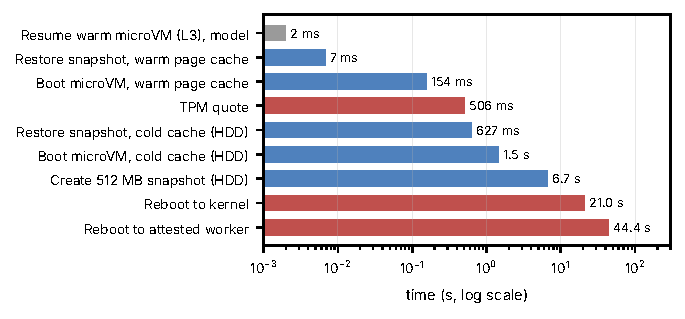
\includegraphics[width=\columnwidth]{figures/fig_cost}
\caption{Time to reach each state on the calibration machine (log scale). Blue: sandbox start-up; red: establishing an
attested worker; grey: model value (not measured). Medians over repeated runs (Section~\ref{sec:calib}).}
\label{fig:cost}
\end{figure}

\subsection{Remote attestation and secret provisioning}
\label{sec:rats}
We use the vocabulary of the IETF RATS architecture \cite{rfc9334}. The \emph{attester} is the volunteer host. During
\emph{measured boot}, each boot stage (firmware, boot loader, kernel image) is hashed into a platform configuration
register (PCR) of the TPM, so the register values are a hash chain of what ran \cite{tcg2019tpm}. On request the TPM
signs selected PCR values together with a verifier-chosen nonce using an attestation key; this signed object is the
\emph{quote}, and the attestation key is certified by the TPM's endorsement key, whose certificate chains to the
manufacturer. The \emph{verifier} checks the signature and the certificate chain, replays the event log against
\emph{reference values} for known-good software, and issues an \emph{attestation result}. A \emph{relying party}, here the
tenant's \emph{key broker service} (KBS), releases a secret only to an attester with an acceptable result
\cite{schear2016keylime}. Two properties matter for scheduling. A quote shows what software booted at one moment, so
evidence goes stale and must be refreshed. And attestation says nothing about \emph{availability}: a host that
passes attestation can still stop working.

\subsection{Volunteer hosts and failure model}
A volunteer host alternates between off and a \emph{session}: an interval during which it is booted into the platform. Session
lengths are heavy-tailed and depend on the time of day \cite{javadi2013fta}. A session ends gracefully with advance notice or
abruptly (reboot, power loss), sometimes for a whole city at once. We use the standard classification of failures into
crash, omission, timing and Byzantine \cite{cristian1991understanding,avizienis2004basic}. An \emph{omission failure}
is a host that does not send a result it owes; a \emph{timing failure} sends it too late. Churn produces crashes; an adversarial owner who
cannot forge or tamper can still choose \emph{when} to omit or delay, selectively and while keeping liveness signals
healthy. Such \emph{gray failures}, where a component appears healthy to simple probes but fails applications
\cite{huang2017gray}, defeat heartbeat-based detectors, including accrual detectors \cite{hayashibara2004phi}.

\subsection{Problem statement and goals}
\textbf{Input.} A stream of invocations, each with a tenant, function, service class (synchronous, asynchronous, or
preemptible filler), deadline, input size and an idempotence flag, arriving from geo-distributed clients; and a dynamic population
of volunteer hosts, each with slots, memory and disk budgets, a location and failure domain, a trust substrate, and a
session that can end at any time. \textbf{Decisions.} Which hosts to attest-and-provision for which tenants, which functions to keep at
which start-up tier on which hosts, and which host runs each invocation (possibly hedged by a duplicate).
\textbf{Objectives.} Meet each class's latency SLO (success rate, deadline-met fraction, P99 of synchronous invocations),
while limiting donor resources (memory held warm), \emph{key exposure} (Section~\ref{sec:exposure}), and wasted work.

We pursue four goals.
\begin{description}
\item[G1] \emph{Confidentiality and integrity.} A malicious owner learns no tenant secret and forges no result.
\item[G2] \emph{Latency under churn.} Tail latency stays within the SLO although sessions end at any time.
\item[G3] \emph{Liveness under omission.} A host that accepts work and discards it, or a scheduler that stalls, is detected and
bypassed within seconds, without trusting liveness signals.
\item[G4] \emph{Verifiable accounting.} Contributed work is recorded so that a host cannot claim work it did not do.
\end{description}
\textbf{Non-goals.} We do not defend against physical attacks on the TPM, vulnerabilities in the appliance
itself, side channels, or failure of the provider-operated control plane (Section~\ref{sec:threat}). We treat invocations as independent; function workflows (DAGs) are discussed in Section~\ref{sec:dag}.
